%\documentclass[a4paper,10pt]{article}
\documentclass[a4paper]{article}
%\usepackage[paper=a4paper, hmargin=0.5cm, bottom=0.5cm, top=0.5cm]{geometry}
\usepackage[latin1]{inputenc}
\usepackage[T1]{fontenc}
\usepackage[spanish]{babel}
\usepackage{xspace}
\usepackage{xargs}
\usepackage{ifthen}
\usepackage{listings}
\usepackage{aed2-symb,aed2-itef,aed2-tad,caratula}
\usepackage{xcolor}
\usepackage{listings}
\usepackage{soul}

%lo agregue yo
\usepackage{graphicx}
\graphicspath{ {imagenes/} }
\usepackage{pgfplots}
\usepackage{tikz}

\usepackage[T1]{fontenc}
\usepackage{inconsolata}

\usepackage{color}

\definecolor{pblue}{rgb}{0.13,0.13,1}
\definecolor{pgreen}{rgb}{0,0.5,0}
\definecolor{pred}{rgb}{0.9,0,0}
\definecolor{pgrey}{rgb}{0.46,0.45,0.48}

\usepackage{listings}
\lstset{language=Java,
  showspaces=false,
  showtabs=false,
  breaklines=true,
  showstringspaces=false,
  breakatwhitespace=true,
  commentstyle=\color{pgreen},
  keywordstyle=\color{pblue},
  stringstyle=\color{pred},
  basicstyle=\ttfamily,
  moredelim=[il][\textcolor{pgrey}]{$$},
  moredelim=[is][\textcolor{pgrey}]{\%\%}{\%\%}
}

\usepackage[latin1]{inputenc} 
\usepackage{multirow}

\newcommand{\moduloNombre}[1]{\textbf{#1}}
\newcommand{\bigO}{\mathcal{O}}
\newcommand{\complejidad}[2]{\hfill $#1 \bigO(#2)$}

\let\NombreFuncion=\textsc
\let\TipoVariable=\texttt
\let\ModificadorArgumento=\textbf
\newcommand{\res}{$res$\xspace}
\newcommand{\tab}{\hspace*{7mm}}

\newcommandx{\TipoFuncion}[3]{%
\NombreFuncion{#1}(#2) \ifx#3\empty\else $\to$ \res\,: \TipoVariable{#3}\fi%
}
\newcommand{\In}[2]{\ModificadorArgumento{in} \ensuremath{#1}\,: \TipoVariable{#2}\xspace}
\newcommand{\Out}[2]{\ModificadorArgumento{out} \ensuremath{#1}\,: \TipoVariable{#2}\xspace}
\newcommand{\Inout}[2]{\ModificadorArgumento{in/out} \ensuremath{#1}\,: \TipoVariable{#2}\xspace}
\newcommand{\Aplicar}[2]{\NombreFuncion{#1}(#2)}

\newlength{\IntFuncionLengthA}
\newlength{\IntFuncionLengthB}
\newlength{\IntFuncionLengthC}
%InterfazFuncion(nombre, argumentos, valor retorno, precondicion, postcondicion, complejidad, descripcion, aliasing)
\newcommandx{\InterfazFuncion}[9][4=true,6,7,8,9]{%
  \hangindent=\parindent
  \TipoFuncion{#1}{#2}{#3}\\%
  \textbf{Pre} $\equiv$ \{#4\}\\%
  \textbf{Post} $\equiv$ \{#5\}%
  \ifx#6\empty\else\\\textbf{Complejidad:} #6\fi%
  \ifx#7\empty\else\\\textbf{Descripci\'on:} #7\fi%
  \ifx#8\empty\else\\\textbf{Aliasing:} #8\fi%
  \ifx#9\empty\else\\\textbf{Requiere:} #9\fi%
}

\newenvironment{Interfaz}{%
  \parskip=2ex%
  \noindent\textbf{\Large Interfaz}%
  \par%
}{}

\newenvironment{Representacion}{%
  \vspace*{2ex}%
  \noindent\textbf{\Large Representaci\'on}%
  \vspace*{2ex}%
}{}

\newenvironment{Algoritmos}{%
  \vspace*{2ex}%
  \noindent\textbf{\Large Algoritmos}%
  \vspace*{2ex}%
}{}


\newcommand{\titlex}[1]{
  \vspace*{1ex}\par\noindent\textbf{\large #1}\par
}

\newenvironmentx{Estructura}[2][2={estr}]{%
  \par\vspace*{2ex}%
  \TipoVariable{#1} \textbf{se representa con} \TipoVariable{#2}%
  \par\vspace*{1ex}%
}{%
  \par\vspace*{2ex}%
}%

\newboolean{EstructuraHayItems}
\newlength{\lenTupla}
\newenvironmentx{Tupla}[1][1={estr}]{%
    \settowidth{\lenTupla}{\hspace*{3mm}donde \TipoVariable{#1} es \TipoVariable{tupla}$($}%
    \addtolength{\lenTupla}{\parindent}%
    \hspace*{3mm}donde \TipoVariable{#1} es \TipoVariable{tupla}$($%
    \begin{minipage}[t]{\linewidth-\lenTupla}%
    \setboolean{EstructuraHayItems}{false}%
}{%
    $)$%
    \end{minipage}
}

\newcommandx{\tupItem}[3][1={\ }]{%
    %\hspace*{3mm}%
    \ifthenelse{\boolean{EstructuraHayItems}}{%
        ,#1%
    }{}%
    \emph{#2}: \TipoVariable{#3}%
    \setboolean{EstructuraHayItems}{true}%
}

\newcommandx{\RepFc}[3][1={estr},2={e}]{%
  \tadOperacion{Rep}{#1}{bool}{}%
  \tadAxioma{Rep($#2$)}{#3}%
}%

\newcommandx{\Rep}[3][1={estr},2={e}]{%
  \tadOperacion{Rep}{#1}{bool}{}%
  \tadAxioma{Rep($#2$)}{true \ssi #3}%
}%

\newcommandx{\Abs}[5][1={estr},3={e}]{%
  \tadOperacion{Abs}{#1/#3}{#2}{Rep($#3$)}%
  \settominwidth{\hangindent}{Abs($#3$) \igobs #4: #2 $\mid$ }%
  \addtolength{\hangindent}{\parindent}%
  Abs($#3$) \igobs #4: #2 $\mid$ #5%
}%

\newcommandx{\AbsFc}[4][1={estr},3={e}]{%
  \tadOperacion{Abs}{#1/#3}{#2}{Rep($#3$)}%
  \tadAxioma{Abs($#3$)}{#4}%
}%

\usepackage{pdfpages}

\begin{document}

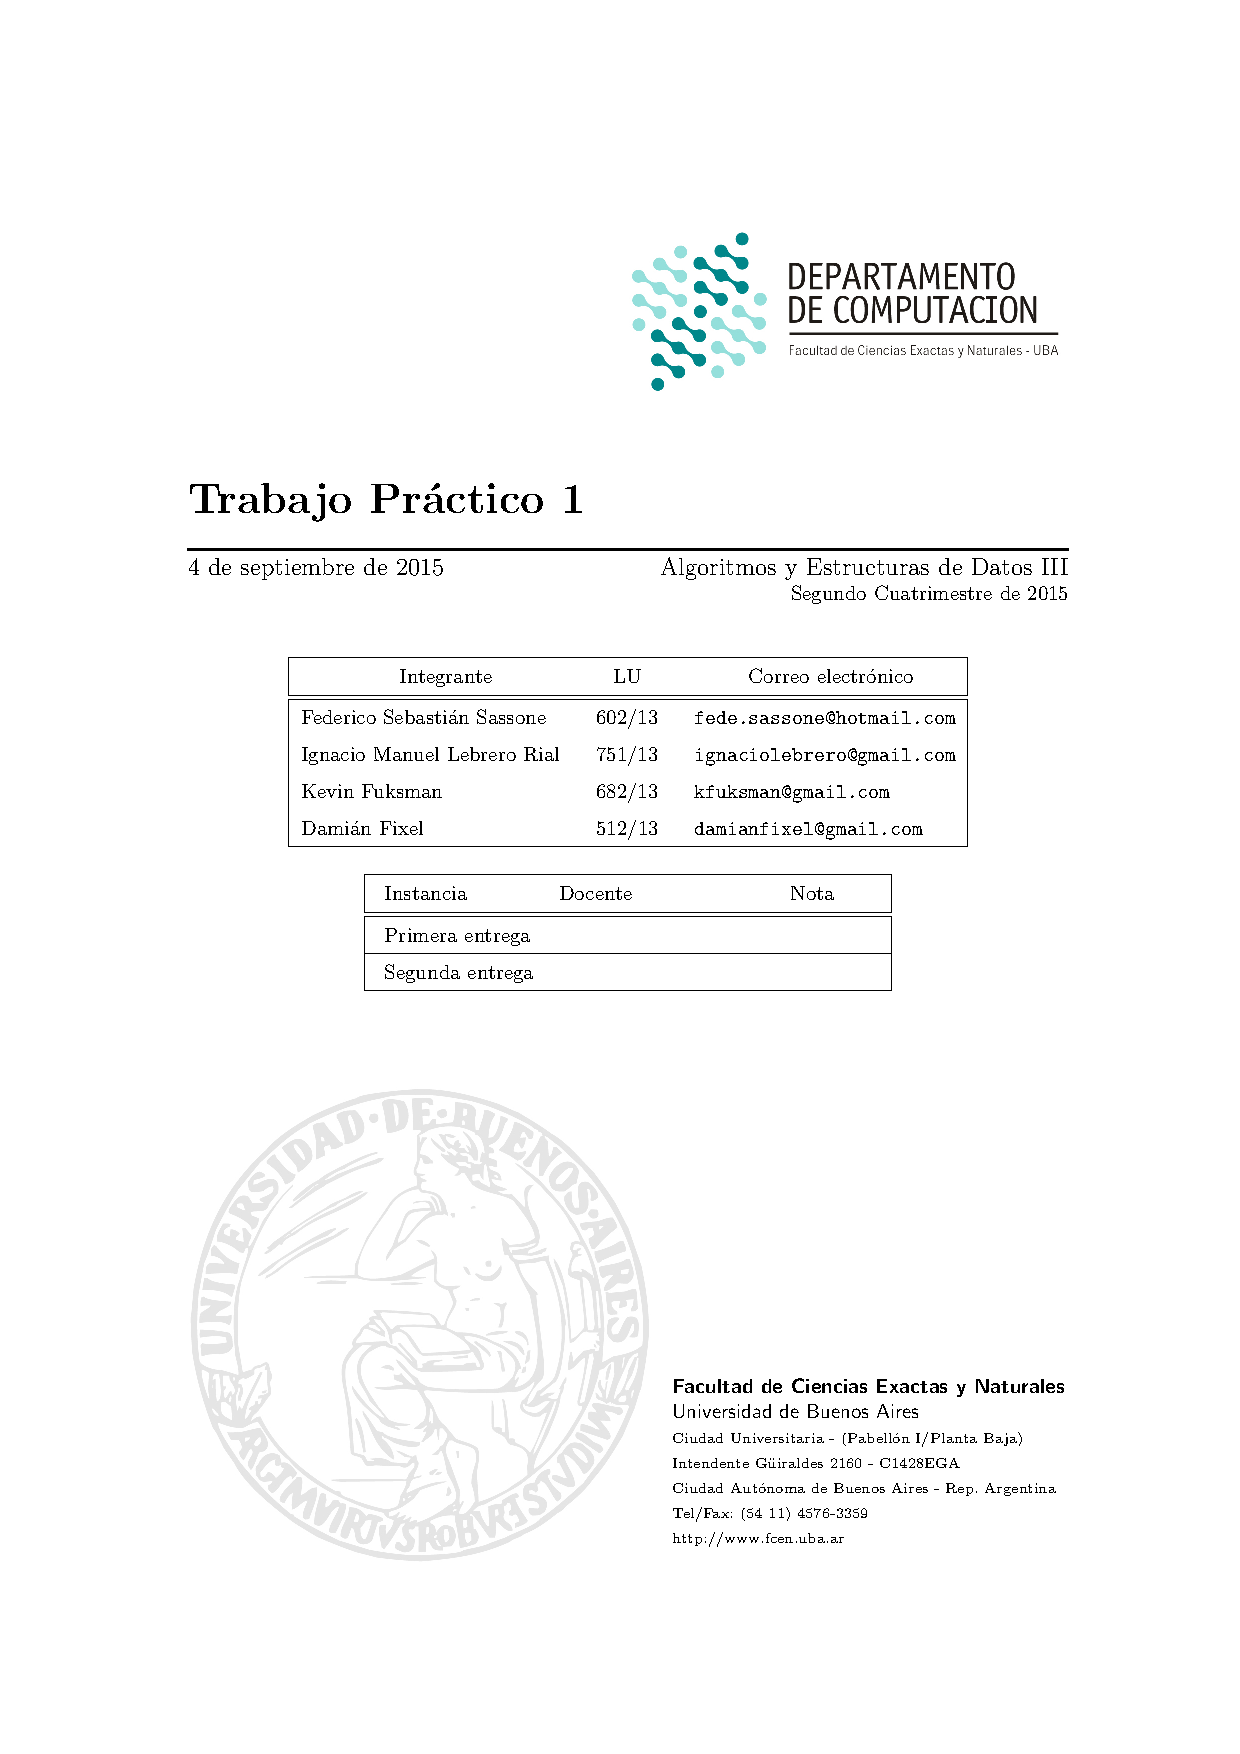
\includepdf{caratula}

% compilar 2 veces para actualizar las referencias
\tableofcontents

\pagebreak
\section{Ejercicio 1}
\subsection{Problema: Tel\'egrafo}

La comunicacion es el progreso! decididos a entrar de lleno en la nueva era el pais decidio conectar telegraficamente todas las estaciones del moderno sistema ferreo que recorre el pais en abanico con origen en la capita (el kilometro 0). Por lo escaso del presupuesto, se ha decidido ofrecer cierta cantidad de kilometros de cable a cada ramal. Pero para maximizar el impacto en epocas electorales se busca lograr conectar la mayor cantidad de ciudades con los metros asignados (sin hacer cortes en el cable).\\

 Se busca optimizar las conexiones entre estaciones de un sistema de trenes. Para esto contamos con los siguientes datos:\\   
 
 El sistema est\'a dividido en ramales.
 
 Cada ramal comienza en la capital, que se encuentra en el kil\'ometro 0.
 
 En cada ramal contamos con una cantidad de cable para conectar estaciones.
 
 Se busca conectar la mayor cantidad de estaciones para cada ramal, sabiendo que el cable conector no puede dividirse.\\
 
 Se nos pide devolver por cada ramal un entero con la cantidad m\'axima de estaciones conectables respetando la complejidad $\bigO (n)$ siendo $n$ la cantidad de estaciones del sistema.

\subsubsection{Ejemplos}

\begin{table}[htb]
\centering
\begin{tabular}{|l|c|}
\hline
\multicolumn{1}{|c|}{Lineas Entrada}  & \multicolumn{1}{l|}{Linea Salida} \\ \hline
6                                     & \multirow{2}{*}{3}                \\ \cline{1-1}
6 8 12 15                             &                                   \\ \hline
35                                    & \multirow{2}{*}{6}                \\ \cline{1-1}
8 14 20 40 45 54 60 67 74 89 99       &                                   \\ \hline
100                                   & \multirow{2}{*}{4}                \\ \cline{1-1}
35 87 141 163 183 252 288 314 356 387 &                                   \\ \hline
90                                    & \multirow{2}{*}{14}               \\ \cline{1-1}
6 8 16 19 28 32 37 45 52 60 69 78 82  &                                   \\ \hline
4                                     & \multirow{2}{*}{0}                \\ \cline{1-1}
5 13 19 26 35                         &                                   \\ \hline
5                                     & \multirow{2}{*}{2}                \\ \cline{1-1}
5 13 19 26 35                         &                                   \\ \hline
5                                     & \multirow{2}{*}{2}                \\ \cline{1-1}
7 16 19 27 33                         &                                   \\ \hline
8                                     & \multirow{2}{*}{4}                \\ \cline{1-1}
2 5 8 14 18                           &                                   \\ \hline
8                                     & \multirow{2}{*}{3}                \\ \cline{1-1}
3 6 9 15 19                           &                                   \\ \hline
\end{tabular}
\caption{Ejemplos Tel\'egrafo}
\label{my-label}
\end{table}


\pagebreak
\subsection{Desarrollo}


 Para comenzar, tengamos en cuenta que el cable no puede dividirse, es decir que las estaciones conectadas deben ser consecutivas. Sabiendo esto, encaramos el problema mediante un algoritmo goloso.
 
 
 La idea es conectar todas las estaciones consecutivas posibles en un arreglo hasta que no tengamos mas cable disponible.\\
 
 Comenzamos recorriendo las estaciones pasadas por par\'ametro en orden, partiendo de una estaci\'on central imaginaria en el kilometro 0 y conectando cada una con su siguiente.
 
 Cuando decimos que $"conectamos"$ una estaci\'on con la siguiente, lo que hacemos en realidad es restarle al cable disponible la distancia entre ambas (su distancia es a la vez la resta entre el entero que representa a la estaci\'on siguiente menos el entero que representa a la estaci\'on actual).
 
 Si recorremos todas las estaciones con el cable disponible, devolveremos la cantidad total de estaciones mas uno (por la estaci\'on central); si esto no sucede es porque nos quedamos sin cable, es decir a la hora de conectar una estaci\'on con la siguiente, la distancia entre ambas fue mayor al cable restante.
 
 Cuando esto ocurra, tendremos que verificar que obtuvimos la mayor cantidad de estaciones conectables de la siguiente forma:
 
 Guardar la m\'axima cantidad de estaciones conectables obtenida hasta ahora y desconectar la primer estaci\'on del arreglo para asi intentar conectar la proxima estaci\'on (si es que existe) con el cable ahora sobrante despu\'es de desconectar la primera del arreglo.
 
 Si la distancia a la proxima estaci\'on (si es que existe) es mayor al cable restante, seguiremos desconectando de a una las estaciones del arreglo (siempre desconectando la primera) para obtener m\'as cable y reintentar conectar.\\
 Puede ocurrirr que la distancia a la pr\'oxima estaci\'on a conectar sea mayor que la cantidad de cable disponible (inclusive luego de desconectar todas las del arreglo). Si esto sucede, comenzaremos a completar el arreglo con el mismo metodo partiendo desde esta estaci\'on.\\
 
 Cuando lleguemos a la \'ultima estaci\'on, devolveremos el m\'aximo entre la cantidad de estaciones en el arreglo de estaciones conectadas actual y la m\'axima cantidad que fuimos guardando cada vez que nos qued\'abamos sin cable.
 
 
\pagebreak

\subsection{Justificaci\'on y Complejidad}

 Utilizaremos dos sub\'indices para recorrer las estaciones del problema. Ambos comienzan seteados en 0, o sea en la posici\'on de la estaci\'on central. Uno corresponde a la primera estaci\'on conectada en el arreglo actual de estaciones conectadas, $(A)$, y otro a la \'ultima estaci\'on conectada o agregada al arreglo de estaciones conectadas, $(B)$. 
 
El algoritmo termina cuando el \'indice $(B)$ llega a la \'ultima estaci\'on. Esto puede ocurrir de varias maneras y aunque el algoritmo tiene complejidad lineal, hay un mejor y peor caso:

\begin{enumerate}
    \item O bien la cantidad de cable inicial alcanz\'o para recorrer todas las estaciones y el algoritmo termina luego de hacer n conexiones.
    \subitem Este es el mejor caso ya que se recorren las n estaciones y se devuelve la mayor cantidad conectable en $\bigO(n)$.
    
    \item O se hacen uno o m\'as guardados de la m\'axima cantidad de estaciones conectadas actualmente y se comienza con un nuevo arreglo de estaciones conectadas.
    
    \subitem Este es el peor caso; ya que si bien el problema se resuelve en tiempo lineal $\bigO(n)$, se realizan hasta el doble de operaciones que en el caso anterior. 
\end{enumerate}
    
Veamos el peor caso posible: \\
    
     Imaginemos que tenemos n estaciones: n-1 estaciones en los kil\'ometros {1,2...n-1} y la \'ultima en el kil\'ometro  2n. Tambien supongamos que tenemos n kil\'ometros de cable. Nuestro algoritmo conectar\'ia las estaciones 1 a n-1 en n-1 pasos. Sin embargo, cuando intente conectar n-1 con n, tardar\'a n pasos en ver que es imposible; para luego comenzar otro arreglo en la \'ultima estaci\'on de la entrada de par\'ametros y terminar.\\


A continuaci\'on analizaremos el algoritmo:
\begin{description}
    Algoritmo 1.1 - Vista general - parametros: estaciones[], cableRestante
    \begin{verbatim}
    FOR i desde 1 hasta estaciones.length()  // O(n)
        distanciaActual = estaciones[i] - estaciones[i-1] //  O(1)
    
        IF cableRestante - distanciaActual >= 0
            .
            Algoritmo 1.2
            .
        ELSE
            .
            Algoritmo 1.3
            .
        ENDIF
    ENDFOR
    IF max > 0 : // O(1)
        max++  // O(1)
    ENDIF
    \end{verbatim}
\end{description}    
    
El bucle general recorre el arreglo linealmente, por lo que hasta el momento lleva $\bigO(n)$.
Veamos que ocurre en el algoritmo 1.2:

\begin{description}
    Algoritmo 1.2
    \begin{verbatim}
        cableRestante -= distanciaActual  // O(1)
        cantEstaciones++  // O(1)
        max = maximo(max, cantEstaciones) //  O(1)
        ultimaEstacionSumo[i-1] = true //  O(1)
        i++;  O(1)
    \end{verbatim}
\end{description}

En el caso de que con el cable que tenemos podamos agregar la proxima estaci\'on, simplemente se agrega y se resta al cable.
La complejidad de este caso es $\bigO(1)$ por lo que hasta el momento seguimos teniendo $\bigO(n)$

veamos el algoritmo 1.3:
\begin{description}
    Algoritmo 1.3
    \begin{verbatim}
         WHILE cableRestante - distanciaActual <= 0 && ultimaEstacion < i // O(n)
            IF ultimaEstacionSumo[ultimaEstacion] // O(1)
                distanciaASacar = estaciones[ultimaEstacion+1] -
                estaciones[ultimaEstacion]  // O(1)
                
                cableRestante += distanciaASacar // O(1)
                cantEstaciones-- // O(1)
            ENDIF
            ultimaEstacion++ // O(1)
        ENDWHILE
        IF ultimaEstacion == i // O(1)
            i++ //  O(1)
        ENDIF
    \end{verbatim}
\end{description}

a simple vista parece ser $\bigO(n)$ este caso, con lo que quedaria peor caso $\bigO(n^2)$ la soluci\'on, pero observando la condici\'on del bucle podemos ver que pide $ultimaEstacion < i$ por lo que no ira mas alla del indice en el que se encuentre el bucle exterior(algoritmo 1.1) y la variable $ultimaEstacion$ siempre avanza, por lo tanto este bucle hara como mucho $n$ pasos en el tiempo total en que corra el algoritmo. dado que es sobre el total de tiempo de corrida del algoritmo 1.1 lo tomaremos como una suma con respecto al bucle exterior, con esto la complejidad queda:\newline

\begin{center}
    $\bigO(n + n)$ \newline \newline
    $\bigO(2n)$ \newline \newline
    $\bigO(n)$ \newline \newline
\end{center}

Que es lo que queriamos demostrar.

\subsection{Correctitud}     
Probemos el algoritmo por inducci\'on \newline
Quiero probar P(n) = $(\forall n : entero > 0$) mi algoritmo devuelve la mayor cantidad de las n+1 estaciones consecutivas que se puedan conectar con una distancia de cable determinada o de no poder hacerlo devuelva cero. \newline
Veamos el caso base, n=1: \newline
resto estaciones[1] con estaciones[0] y pregunto si el cable alcanza.\newline

\begin{enumerate}
    \item De alcanzar (algoritmo 1.2) agrego esa estaci\'on y pasa a ser la mas larga hasta el momento, luego termina el agoritmo ya que no vuelve a cumplir la condici\'on del algoritmo 1.1. El resultado son dos estaciones. \newline
    \item De no alcanzar (algoritmo1.3) entro en el bucle, la primera condici\'on se cumple autom\'aticamente por hip\'otesis de este caso, y como entra con i = 1, \'ultima estaci\'on ser\'a 0, por lo que la condici\'on da true y pasa. Como el arreglo ultimaEstacion empieza en false, no se cumple la condici\'on y paso a sumar a ultimaEstacion, como esta es igual a i sumo 1 a i y vuelvo al bucle exterior. En este momento la condici\'on no se cumple y sale, dando como resultado cero estaciones. 
\end{enumerate}

Con esto queda probado que el caso base funciona, nuestra hip\'otesis inductiva sera que mi algoritmo funciona para $p(n)$, ahora suponiendo que vale $p(n)$ veamos si vale para $p(n+1)$.\newline \newline
Primero podemos observar que el arreglo contiene $n+2$ elementos, los cuales pueden ser tomados como un arreglo de $n+1$ elementos concatenado con el elemento $n+2-esimo$, sabiendo esto puedo aplicar mi hip\'otesis inductiva sobre el arreglo de $n+1$ elementos y comenzar la demostraci\'on en el elemento $n+2-esimo$ en el algoritmo 1.1, por hi\'potesis inductiva hasta el momento $\exists\ s : entero$ una posible soluci\'on maxima que conecta $k$ estaciones, con $0<= k <= n$ y hay una cantidad de cable dispnible $m$ con $0<= m <= cablemaximo$. sigamos con el algoritmo: \newline

El elemento entra al bucle del algoritmo 1.1, pasa ya que es el ultimo elemento, calculo la distancia entre la $n+1-esima$ y $n+2-esima$ estaciones, ahora:
\begin{enumerate}
    \item Si es menor a $m$, agrego esta estaci\'on, sumo uno mas y en la proxima iteracion salgo: \newline
    \begin{enumerate}
    \item si el maximo local que se estaba calculando hasta la anterior iteracion mas la nueva estaci\'on es mayor a $s$, entonces el maximo sera el maximo local mas uno, ya que agregue la nueva estaci\'on.
    \item si el maximo local que se estaba calculando hasta la anterior iteracion mas la nueva estaci\'on es menor o igual $s$, entonces el maximo sera $s$.
    \end{enumerate}
    
    \item si no, entro en el else y comienzo a sacar estaciones del princio de la subsolucion actual:
    \begin{enumerate}
    \item Si saco todas las estaciones que tenia hasta el momento, me quedara solo la nueva estaci\'on que agregue, con lo que significa que no me alcanza el cable, suma uno a i y en la proxima iteracion del algoritmo 1.1 no entrara en el bucle principal, devolviendo el resultado $s$ previamente calculado.
    \item Si saco algunas de las estaciones que tenia hasta el momento, me quedara un subarreglo de estaciones y al salir del bucle, volvera a entrar en el algoritmo 1.1 entrando por la primer condici\'on y caera en el caso 1 de esta demostracion.
    \end{enumerate}
\end{enumerate}
Con esto vale $P(n+1)$. Luego $(\forall\ n : entero > 0$) mi algoritmo devuelve la mayor cantidad de las n+1 estaciones consecutivas que se puedan conectar con una distancia de cable determinada o de no poder hacerlo devuelve cero.\newline
Con esto queda demostrado que el algoritmo es correcto.

\subsection{Tests}
Para los Tests analizamos su mejor y peor caso.
    \subsubsection{Mejor Caso}
        El mejor caso es que nunca tenga que sacar estaciones de la subsolucion que este calculando, para esto armamos un arreglo cuya suma de distancias sea menor a la longitud maxima de cable, de esta manera siempre agrega siendo costo $\bigO(n)$. \newline
    \lstinputlisting[language=Java]{modulos/Tests_Code/testej1mejor.txt}
    
    \subsubsection{Peor Caso}
        El peor caso es cuando debe sacar todas las estaciones del arreglo ya que termina siendo costo $2 * \bigO(n)$, para esto armamos arreglos en donde la distancia entre todas las estaciones sea menor que la longitud total de cable excepto la ultima, cuya logitud es mayor que todo el cable, de esta manera, el algoritmo tendra que realizar 2*n operaciones. \newline
    \lstinputlisting[language=Java]{modulos/Tests_Code/testej1mejor.txt}
    
    \pagebreak
    
    \subsubsection{Performance}
    
    Observamos el contraste de nuestro peor y mejor caso. La variaci\'on en el peor caso est\'a en la constante 2 que multiplica a la cantidad de operaciones realiza en el mejor caso.
    
    \begin{figure}[h!]
    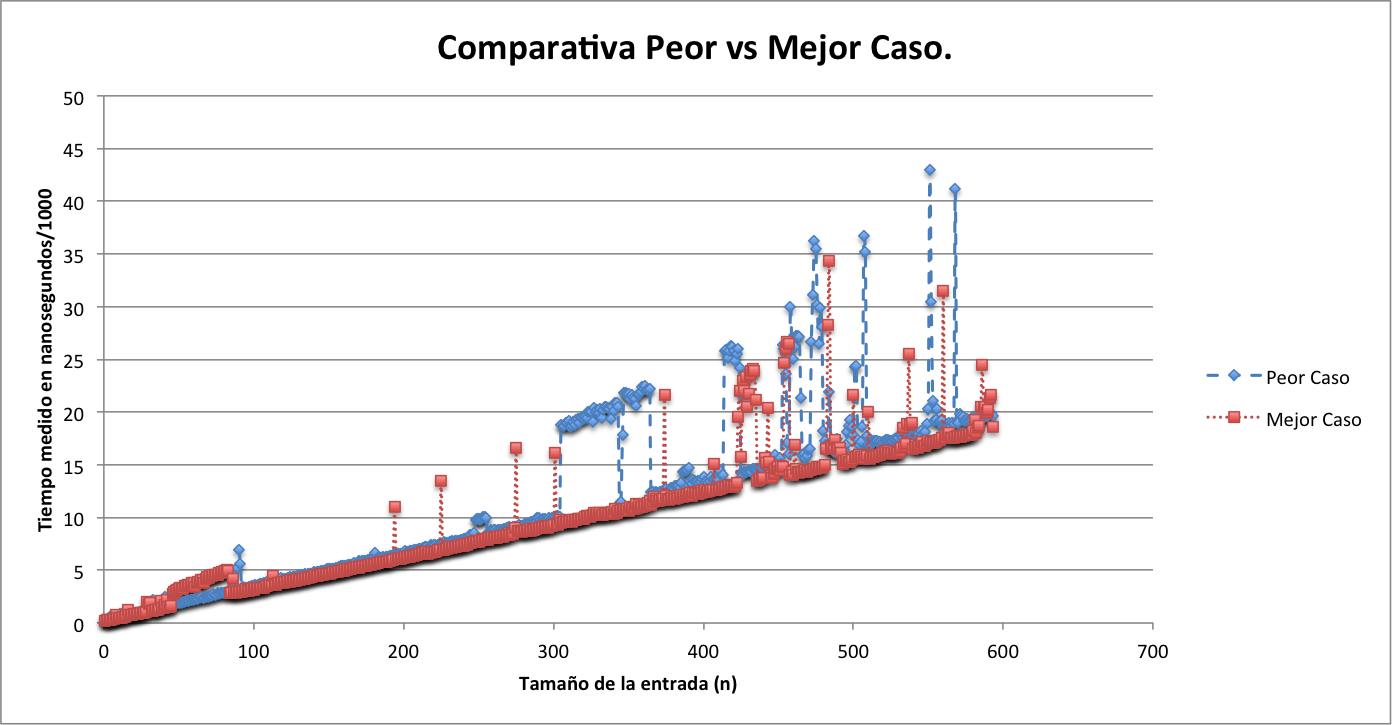
\includegraphics[width=140mm]{ejercicio1_mejorvspeor.png}
    \centering
    \caption{Comparativa Mejor vs Peor Caso}
    \label{overflow3}
    \end{figure}
    
        Se observa que nuestro mejor caso tiene un comportamiento lineal y mantiene ese comportamiento a medida que las entradas se hacen m\'as numerosas. 
    
    \begin{figure}[h!]
    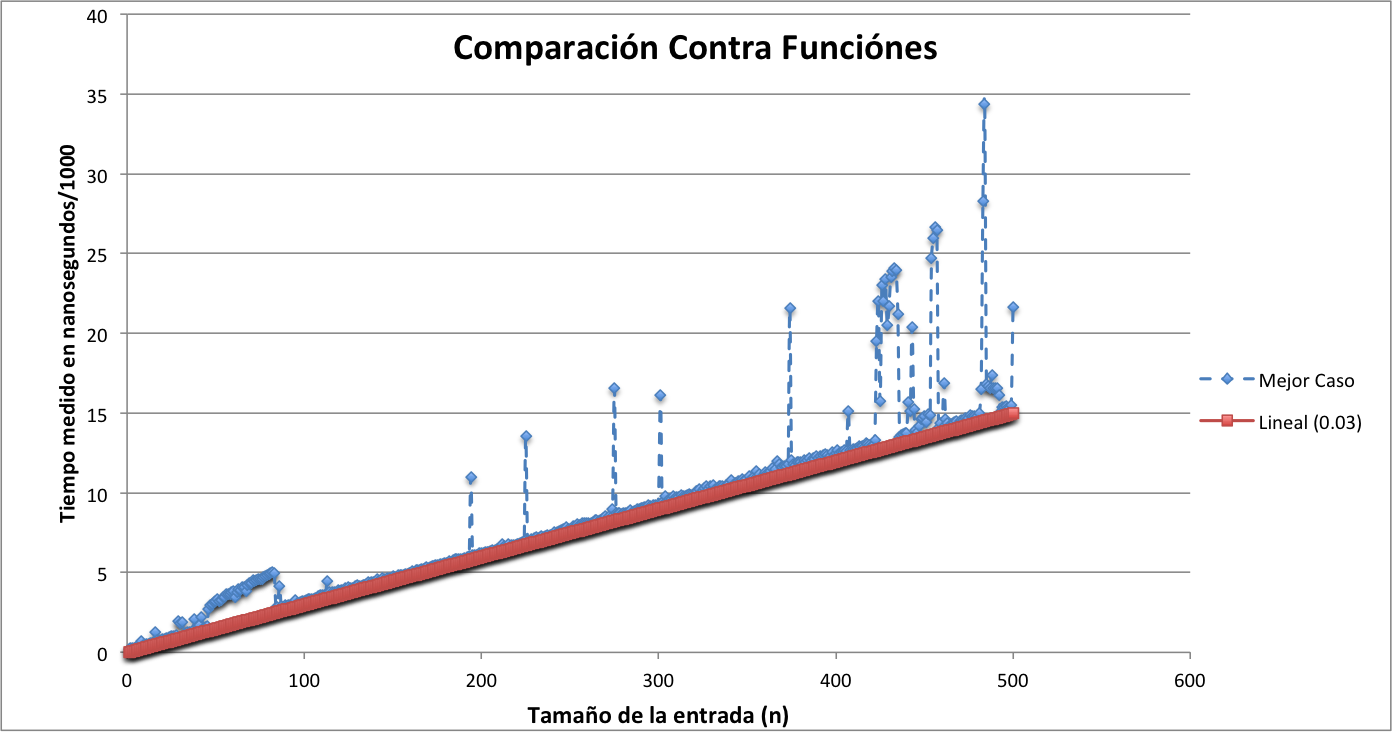
\includegraphics[width=140mm]{ejercicio1_comparativo.png}
    \centering
    \caption{Comparativa Contra Funcion Lineal, Cuadratica y constante}
    \label{overflow3}
    \end{figure}

\pagebreak
\pagebreak
\pagebreak
\section{Ejercicio 2}

\subsection{Problema: A Medias}
 Nos proveen la defici\'on de mediana de un conjunto ordenado de $n$ elementos como: \\
 $x_{(n+1)/2}$ si $n$ es impar \\
 $(x_{n/2} + x_{n/2+1)} /2$ si $n$ es par.\\
 
 Se nos pide dada una entrada de $n$ n\'umeros enteros no ordenados devolver otros $n$ n\'umeros donde el $i$\'esimo de ellos represente la parte entera de la funci\'on mediana aplicada a los primeros $i$ n\'umeros de la entrada, luego de ser ordenados. \\
 Adem\'as la resoluci\'on de este problema debe obtenerse en una complejidad estrictamente menor a $\bigO (n²)$ siendo $n$ el n\'umero total de enteros en la entrada.\\
 Luego, la entrada ser\'a una linea de $n$ n\'umeros, al igual que la salida.
\subsubsection{Ejemplos}


\begin{table}[htb]
\centering
\begin{tabular}{|l|l|}
\hline
Linea Entrada     & Linea Salida      \\ \hline
2 3 4 1 2         & 2 2 3 2 2         \\ \hline
2 7 2 8 4 9 1 6 5 & 2 4 2 4 4 5 4 5 5 \\ \hline
1 87 4            & 1 44 4            \\ \hline
4 0 32 6 8 10     & 4 2 4 5 6 7       \\ \hline
\end{tabular}
\caption{Ejemplos A Medias}
\label{my-label}
\end{table}

\subsection{Desarrollo} 
La complejidad intrinseca de este ejercicio esta en ir recorriendo un vector de n\'umeros, e ir de alguna manera ordenando este nuevo array para obtener f\'acilmente la mediana, que sabemos que si se cumple la anterior propiedad es muy f\'acil calcularlo. 
Para lograr esto hicimos uso de una estructura que nos permite obtener el valor del m\'inimo/m\'aximo barato y la insercion y borrado relativamente tambien.
La idea es mantener siempre la idea de puntero al medio de lo que seria el array actual, por lo que decidimos usar un minHeap, un maxHeap y una variable, lo que hace que nuestro array se convierta en la siguiente estructura. \\

\begin{center}
    [1 , 2 , 3 , 4 , 5] 
\end{center}\\

\begin{center}
    maxheap(1,2)  ++  3  ++ minHeap(4,5) 
\end{center}

La idea del "++"\ es que si vamos extrayendo el maxheap incrementando las posiciones , agregamos la variable del medio y luego extraemos el minHeap volvemos a obtener nuestro array inicial, este vendria a ser nuestro funcion de Abstraccion que matchea nuestra estructura con un array convencional.

Teniendo esta estructura es muy f\'acil ir agregando nuevos elementos y mantenerla consistente es muy sencillo. La idea es la siguiente:

Si el elemento nuevo es menor a la variable (esta es el "medio"), se agrega al maxHeap, caso contrario se la agrega al minHeap. Luego de esto se llama a una funcion que readjusta la estructura de ser necesario para luego simplemente, si el vector es de tama\~no par, se devuelve la suma de la variable mas el min/max del heap que tenga mas elementos, caso contrario se devuelve la variable.

Esta insercion puede generar la necesidad de ajustar la estructura, pero como veremos en la siguiente seccion esto a lo sumo necesita realizar dos pasos. 

\subsection{Justificaci\'on y Complejidad}
El algoritmo crea las estructuras necesarias para trabajar y son las siguientes. \\ \\ 
leftHeap \ \leftarrow \ maxHeap \ de\ tama$\~$no\ n \\
rigthHeap \ \leftarrow \ minHeap \ de\ tama$\~$no\ n \\
resultado  \ \leftarrow \ intArray \ de\ tama$\~$no\ n \\
middle \ \leftarrow intVariable \\

Luego tenemos un for que va a hacer las llamadas correspondientes para resolver el problema.

\begin{description}
    Algoritmo 2.1
    \begin{verbatim}
    FOR i desde 0 hasta n
        resultado[i] <- calcularMediana(array[i],i)
    ENDFOR
    \end{verbatim}   
\end{description}
Aca ya empezamos a observar que el costo de esta funcion al menos va a tener como cota $\bigO (n)$, ya que a lo sumo vamos a recorrer 1 vez el array entero pero nos falta analizar el costo de la funci\'on calcularMediana, por lo tanto la complejidad que podemos asegurar por ahora es $\bigO (n * \bigO(calcularMediana))$ \\ \\

Para analizar la funci\'on anterior vamos a dividirlo en 3 partes, pero antes debemos asegurarnos que las operaciones que utilicemos en los Heaps sean de la complejidad que afirmamos que son.

Para esto fuimos a la documentaci\'on oficial de oracle, en donde citamos la siguiente frase :

"Implementation note: this implementation provides O(log(n)) time for the enqueing and dequeing methods (offer, poll, remove() and add);"

Y la misma fue extraida del siguiente link:\\
\hypertarget{http://docs.oracle.com/javase/7/docs/api/java/util/PriorityQueue.html}

Luego de esta aclaracion podemos continuar con el analisis de las funciones, la interfaz de calculateMediana es :\\
int calculateMediana(int number, int i).


\begin{description}
  \item[Agregar nuevo elemento:] \hfill \\
  Esta seccion es la encargada de ingresar un nuevo elemento, para luego poder mas adelante calcular la mediana del array el cual deberiamos calcular. El pseudo-codigo es bastante sencillo, ya que tenemos un primer caso, en el cual no hay ningun elemento a\~nadido, es decir la estructura esta vacia, y por lo tanto la opreaci\'on simplemente consta en asignar la variable middle, caso contrario, debemos ver en que heap deberiamos insertar el elemento, sin temor a descompensar la estructura, ya que luego llamaremos a una funcion encargada de recomponer la misma de ser necesario.
Es importante observar que si ingresa un elemento repetido, y este es igual al middle, por como se armaron los casos, va a ir al rigthHeap, lo que no causaria ningun tipo de inconveniente. 


\begin{description}
    Algoritmo 2.2
  \begin{verbatim}
    IF i == 0 :
        middle <- number O(1) 
    ELSE :
        IF number < middle :
            leftHeap.add(number) // O(log(n))
        ELSE : 
            rigthHeap.add(number) // O(log(n))
        ENDIF 
    ENDIF
    \end{verbatim}
\end{description}
    
Por lo tanto podemos acotar esta seccion de la funci\'on con costo :  $\bigO (log(n))$
  \item[ajustar la estructura:] \hfill \\
  
  Esta seccion es la que se encarga de en otras palabras, hacer valer nuestro invariante de representacion, que es mantener la variable middle en lo que pasando por nuestra funcion de abstraccion es el centro del array, en caso de ser impar y sino uno de los dos elementos del "medio", en caso de ser par.
  
  El pseudo codigo de la funcion es el siguiente:

\begin{description}
    Algoritmo 2.3
  \begin{verbatim}
    IF rigthHeap.size() - leftHeap.size() > 1 :
        leftHeap.add(middle)   // O(log(n))
        middle = rigthHeap.remove()  // O(log(n)) 
    ELSE IF leftHeap.size() - rigthHeap.size() > 1 :
        rigthHeap.add(middle)  // O(log(n))
        middle = leftHeap.remove() // O(log(n))
    ENDIF
  \end{verbatim}
\end{description}
 
 Olvidandonos de que hay casos en los cuales, esta parte de la funcion tenga costo  $\bigO (1)$ \ ya que no entrariamos en ningun caso, si podemos asegurar que en el caso de necesitar relaizar un adjuste, solo vamos a realizar uno, esto se traduce a ejecutar una sola parte del if.
 Vamos a ver que por absurdo estas condiciones no pueden cumplirse simultaneamente:
 
 Sea a = rigthHeap.size() y b = leftHeap.size() .
 
 Asumimos que  : a - b > 1 y queremos llegar a que b - a > 1
 
 Podemos hacer un pasaje de terminos en la primera por lo que nos quedaria : a > b + 1
 
 Y de la segunda sabemos que b > a + 1, por lo tanto si juntamos las inecuaciones nos queda:
 
 b > a + 1 > a > b + 1  \ \   Abs! 
 
 Como llegamos al absurdo de que b > b + 1 podemos concluir que si sucede a - b > 1, no puede suceder b - a > 1 . Esto lo podemos hacer sin perdida de generalidad y vamos a llegar a la misma conclusion.
 
Por lo tanto este analisis no lleva a poder afirmar que una cota para esta seccion es $\bigO (2 * log(n))$, pero si nos lanzamos a calcular la complejidad sin ningun analisis, la complejidad estaria acotada por $\bigO (4 * log(n))$ y como 2 y 4 son constantes llegamos a la cota final de $ \textbf {\bigO (log(n))}$
 
	
  \item[Devolver el resultado:] \hfill \\
  En esta ultima seccion, lo unico que debemos es identificar en que caso de array estamos, es decir par o impar, por lo que el pseudo-codigo seria el siguiente:
\begin{description}
    Algoritmo 2.4
    \begin{verbatim}
        IF (i+1) % 2 == 0) :
            IF (rigthHeap.size() > leftHeap.size()) :
                return ((rigthHeap.peek() + middle) /2) // O(1)
            ELSE :
                return ((leftHeap.peek() + middle) /2) // O(1)
            ENDIF
        ELSE :
            return middle // O(1)
        ENDIF
    \end{verbatim}
\end{description}

La funcion peek, lo que hace es ver el min/max elemento, y esto lo hace en $\bigO (1)$, por lo tanto la complejidad final de esta seccion es $\textbf{\bigO (1)}$ para cualquier caso, de entrada posible.

\end{description}

Sumando todas las complejidades de las tres divisiones que hicimos, nos queda que la funcion calculateMediana tiene una complejidad de $\bigO (log(n))$ .

Al tener resuelta esta parte, podemos completar lo que antes no podiamos asegurar y por lo tanto la complejidad del problema es :\\

${\bigO (n * log(n))$ \\

Y como $\bigO (log(n))$ < $\bigO (n^2)$, podemos concluir que : \\

$\bigO (n * log(n))$ < $\bigO (n^2)$ \\

Por lo tanto nuestro algoritmo cumple con la complejidad pedida.

\pagebreak

\subsection{Correctitud}

Para empezar a mostrar la correctitud de nuestro algoritmo, vamos a escribir nuestro invariante de representacion en un pseudo lenguaje.

\begin{verbatim}
1) FOREACH leftHeap as element:
    element <= middle
ENDFOREACH
2) FOREACH rigthHeap as element:
    element >= middle
ENDFOREACH
3) | rigthHeap.size() - leftHeap.size()| < 2

\end{verbatim}

Suponiendo que este invariante de representacion, es muy f\'acil ver que la solucion va a hacer correcta, por la definicion de mediana.
Veamos que la definicion de mediana, es igual a nuestra funcion de calcular resultado.

\begin{table}[htb]
\centering
\begin{tabular}{|l|l|l|}
\hline
    & Solucion Mediana  &  Solucion Nuestra     \\ \hline
Caso PAR        & (x_{n/2} + x_{n+1/2})/2 &   ((rigthHeap.peek() + middle) /2) V    \\ 
 & &((leftHeap.peek() + middle) /2 ) \\ \hline
Caso IMPAR & x_{(n+1)/2} &   middle \\ \hline

\end{tabular}
\caption{Comparaci\'on de soluciones}
\label{my-label}
\end{table}

Para no ser redundantes con la copia del codigo, vamos a explicar brevemente que en el caso par, al no existir un "medio", nuestra estructura tiene en la variable middle, uno de los 2 "medios", y con observar el tama\~no de los heaps, podemos determinar cual de ellos tiene al otro "medio".

Ahora que sabemos que de nuestro invariante podemos llegar a la solucion pedida, nos queda ver que haciendo la unica operacion posible con este algotirmo que es agregar un nuevo elemento, la estructura sigue manteniendo el invariante al finalizar su ejecuci\'on.

Veamos primero nuestro case base, las estructuras vacias, y nuestra variable middle sin inicializar. Al no haber elementos en ninguno de los 2 heaps , el FOREACH se cumple trivialmente ya que no hay elementos para ver si la condicion que pedimos es valida. y el tercer punto tambien se cumple trivialmente, si no tiene elementos los tama\~nos son 0, por lo tanto la diferencia entre ellos es 0 y menor que 2.

Luego nos queda ver que pasa al agregar un nuevo elemento, la parte 1 y 2 del invariante de Representacion nunca deja de valer. En la seccion anterior, en la parte que titulamos "Agregar nuevo elemento" y que ser\'ia el Algoritmo 2.2 , vemos ese IF hace que los elementos nuevos se agregen respetando nuestros requerimientos, ya que seria la union de los 2 primeros puntos del invariante plasmados a las condiciones que utilizamos.

Nos falta ver que se sigue cumpliendo la tercera, y para esto nos vamos a apoyar en nuestra funcion de readjuste, que es Algoritmo 2.3. Comprobemoslo con un peque\~no ejemplo pero sin perder la generalidad de en que caso estemos.

Para esto vamos a suponer que nuestro variable middle vale j y vamos a agregar un nuevo elemento llamado k, sin perdida de generalidad podriamos suponer  que j < k y ahora tenemos que ver varios casos en los cuales los heaps tienen distintas cantidad de elementos. Para esto vamos a llamar a nuestro factor de balanceo como | rigthHeap.size() - leftHeap.size()| .

  
\begin{description}
\item[CASO 1, FACTOR DE BALANCEO 0:] \hfill \\
    Este caso es trivial, ya que si nuestro factor de balanceo es 0, agregando un elemento en cualquiera de los heaps, y luego recalculando nuestro factor va a hacer 1, por lo tanto menor a 2, es decir cumple el invariante de representacion.

\item[CASO 2, FACTOR DE BALANCEO 1:] \hfill \\
    Que nuestro factor de balanceo sea 1 significa que uno de los heaps tiene un elemento mayor que el otro, por lo tanto podemos llamarlo H. Y ahora nuevamente tenemos dos casos. que el elemento j haya sido agregado a H o no.
    
    
\begin{center}
\begin{description}
\item[CASO 1, j es agregado a H:] \hfill \\
    En este caso H ya tenia un elemento mas, y como le estamos agregando j, el factor de balanceo pasa a ser 2. por lo tanto lo que debemos hacer y lo que hace el algoritmo realiza es un balanceo. Por lo tanto nuestro algoritmo haria las siguientes acciones :
    
    Vamos a llamar a nuestro otro heap T, el distinto de H.
    \begin{verbatim}
    T.add(middle)   // O(log(n))
    middle = H.remove()  // O(log(n)) 
    \end{verbatim}
Por lo tanto podemos ver que antes de hacer estas dos operaciones estabamos en un factor de balanceo 2, pero agregamos un elemento en T y quitamos uno en H. Por lo tanto nuestro nuevo factor de balanceo en caso de haber hecho un rebalanceo pasa a ser de 0.
\item[CASO 1, j no es agregado a H:] \hfill \\
    Si H tenia un elemento mas pero agregamos un nuevo elemento en el heap T, es facil ver que el factor de balanceo vuelve a tener valor 0, por lo tanto no es necesario hacer ningun readjuste, ya que el elemeto mejora el factor por si solo.

\end{description}
\end{center}

\end{description}

factor de balanceo estaba en 1, lo que significa que uno de los 2 heaps, tenia un elemento mas que el otro, para el proposito de esta demostraci\'on vamos a suponer que este es el rigthHeap, ya que sino no se desbaleancearia la estructura, y no podriamos observar lo que queremos demostrar.



\begin{table}[htb]
\centering
\begin{tabular}{|l|l|l|l|l|}
\hline
    & Tama\~no leftHEAP & Tama\~no rigthHEAP  & valor Middle & Balanceo     \\ \hline
Antes de agregar       & 3  &  4 & 5 & 1       \\ \hline
Despues de agregar & 3 & 5 & 5& 2 \\ \hline

\end{tabular}
\label{my-label}
\end{table}

Si entramos a la funcion encargada de ajustar la estructura, es f\'acil notar que vamos a entrar en este if:
\begin{verbatim}
IF rigthHeap.size() - leftHeap.size() > 1 :
        leftHeap.add(middle)
        middle = rigthHeap.remove()
\end{verbatim}

Entonces volvamos a ver como nos queda nuestro cuadro luego de aplicar esta seccion de la funcion:

\begin{table}[htb]
\centering
\begin{tabular}{|l|l|l|l|l|}
\hline
    & Tama\~no leftHEAP & Tama\~no rigthHEAP  & valor Middle & Balanceo     \\ \hline

Despues de agregar & 3 & 5 & 5& 2 \\ \hline
Despues de ajustar & 4  &  4 & m\'inimo(rigthHeap) & 0      \\ \hline
\end{tabular}
\label{my-label}
\end{table}

Hay que destacar que m\'inimo(rigthHeap) es el elemento m\'inimo que se extrajo en el algoritmo, y por eso su tama\~no bajo en 1. 

Luego vemos que la tercera parte del invariante se cumple, sin perder generalidad podemos ver que como en cada iteracion se llama a esta funcion y solo se agrega a un elemento a la vez, nunca vamos a tener una diferencia mayor a 2, por lo tanto el adjuste de mover un elemento desde el que mas tiene hasta el que menos tiene, teniendo el cuidado de hacer la transicion correspondiente para mantener el punto 1 y 2, balancea la estructura y mantiene los tres puntos de nuestro invariante.

Al haber probado que :
\begin{itemize}
\item Una estructura que cumple el invariante de representacion podemos ir a la solucion del problema.
\item Al agregar un elemento a una instancia que cumple el invariante de representacion, nos lleva a otra instancia valida con ese elemento.
\end{itemize}

Podemos concluir que al agregar un nuevo elemento podemos llegar a una instancia valida, que luego podremos convertirla en una solucion del problema.


\subsection{Tests}
Para los Tests analizamos su mejor y peor caso.
    \subsubsection{Mejor Caso}
        El mejor caso es que el primer elemento se el elemento del medio y que la distribucion de la entrada sea (<middle),(>middle),(<middle) ... lo que va a generar que nunca se necesite balancear la estructura quedando cada iteracion con el costo de insertar un nuevo elemento en un heap, y eso nos cuesta: $\bigO(log(n))$. \newline
    \lstinputlisting[language=Java]{modulos/Tests_Code/testej2mejor.txt}
    \subsubsection{Peor Caso}
        El peor caso es cuando la distribucion de la entrada es monotona creciente/decreciente lo que generaria la necesidad de reajustar la estructura siempre luego de la segunda iteracion, y recordemos que el adjuste de la estructura nos cuenta $\bigO(2 * log(n))$ y a esto hay que sumarle el costo que tenemos siempre de agregar el elemento para luego revisar si hay que rebalancear que es $\bigO(log(n))$ , lo que nos da un total de $\bigO(3 *log(n))$ para cada iteracion luego de la segunda.. \newline
 \lstinputlisting[language=Java]{modulos/Tests_Code/testej2peor.txt}
 
\pagebreak

\subsubsection{Performance}

Comparaci\'on de mejor peor caso. Vemos que crecen asint\'oticamente igual, s\'olo que con distintas pendientes. La constante 3 que afecta al peor caso, surge de que en este caso se suma a la misma inserci\'on del mejor caso, dos mas que son causa de mover el middle a un heap, y el heap que tenia mas elementos a middle.

\begin{figure}[h!]
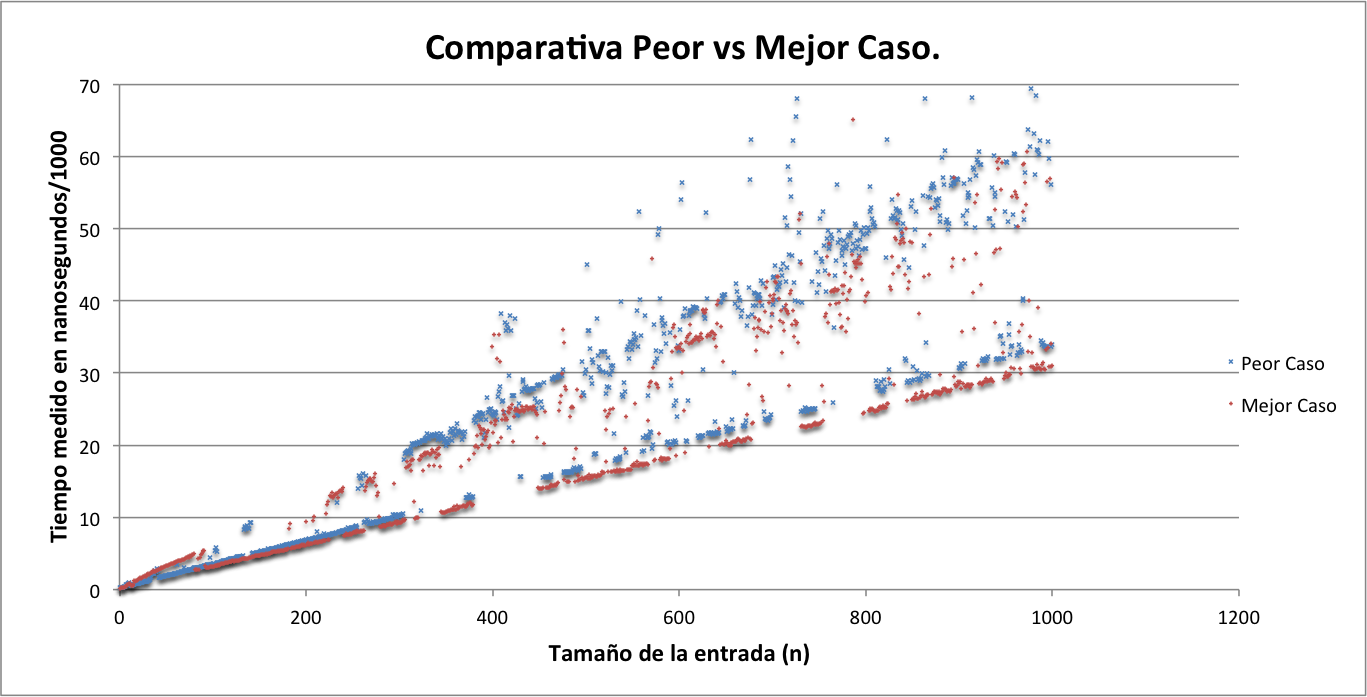
\includegraphics[width=140mm]{ejercicio2_bestVsworst.png}
\centering
\caption{Comparativa Peor vs Mejor Caso}
\label{overflow3}
\end{figure}


Luego podemos ver que la cota que justificamos como  $\bigO(n * log(n))$ est\'a acotada inferiormente por una funci\'on lineal a partir de un n.


\begin{figure}[h!]
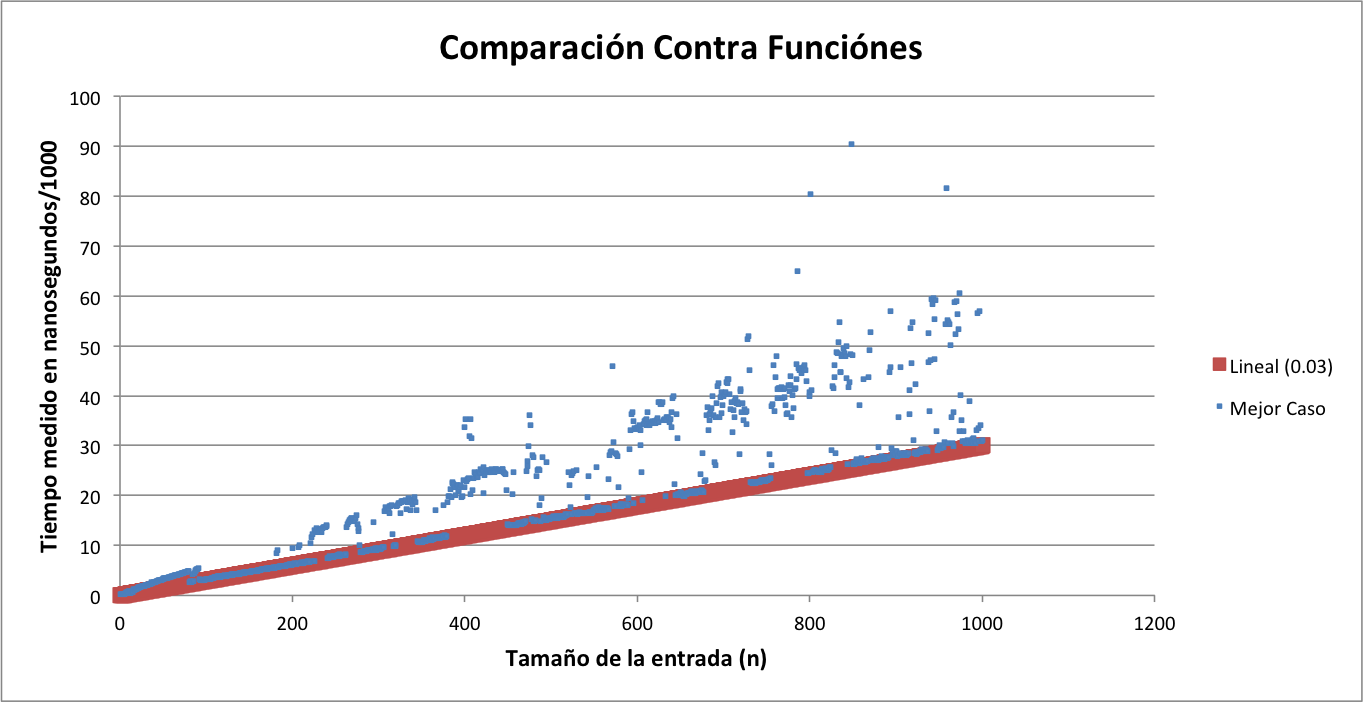
\includegraphics[width=140mm]{ejercicio2_comparacionvsfunciones.png}
\centering
\caption{Comparativa Contra Funcion Lineal y Cuadratica}
\label{overflow3}
\end{figure}


\pagebreak
\section{Ejercicio 3}

\subsection{Problema: Girls Scouts}
El capitan de Las Girasoles quiere evitar los problemas en el fogoon del ano anterior cuando las exploradoras rompieron en llanto por no poder sentarse en la ronda junto a sus mejores amigas. En secreto les asigno una letra a cada nina y relevo quien se llevaba con quien. \\
Su idea es organizar la ronda de manera que exista la menor distancia posible entre cada amistad. \\

Con esto se sabe que trabajara con un conjunto de personas y un conjunto de amistades entre ellos, para esto decidimos modelar al conjunto de personas como un arreglo para determinar las posiciones que tendran cada una. Por otro lado las combinaciones de posibles lugares a saltarce simplemente seran permutaciones del arreglo. \\

La entrada consta de un conjunto de personas y sus respectivas amistades(las cuales tambien perteneceran al conjunto). Se quiere que, al sentarlas a todas en una ronda, se minimize la suma de distancias entre todos los pares de amistades dentro de la misma.
%en tiempo estrictamente menor a $\bigO (e^e . a^2)$ \par

\subsubsection{Ejemplos}

\begin{table}[htb]
\centering
\begin{tabular}{|l|l|}
\hline
Linea Entrada                    & Linea Salida \\ \hline
a bcde;b acde;c abde;d abc;e abc & 2 abdce      \\ \hline
a bcd;b ae;c ad;d ac;e b         & 2 abecd      \\ \hline
a fb;b gc;d gc;f agh;e hd        & 3 abgcdehf   \\ \hline
x yz                             & 1 xyz        \\ \hline
\end{tabular}
\caption{Ejemplos Girls Scouts}
\label{my-label}
\end{table}



\subsection{Desarrollo}
Dado que no es necesario generar las permutaciones que incluyan elementos repetidos, dado $e$ un conjunto de personas, si genero permutaciones con elementos repetidos tendria $e^e$ posibles combinaciones(ya que tendriamos $e$ posibilidades para la primer posicion, $e$ para la segunda y asi hasta la $e-esima$ posicion). A la hora de generar permutaciones sin repeticion de elementos tendremos $e$ posibilidades en la primera posicion, $e-1$ en la segunda y asi susecivamente hasta la llegar a la $e-esima$ posicion donde solo nos quedara una posibildad. De esta manera redujimos el espacio de permutaciones posibles a:
\newline

\begin{center}
    \underline{$e$}
    \underline{$e-1$}
    \underline{$e-2$}
    \underline{$e-3$}
    \underline{$. . .$}
    \underline{$1$} \newline
    Posibles combinaciones \newline \newline
    $= e * (e - 1) * (e - 2) * ... * 1$ \newline \newline
    $= \prod_{i = 1}^e i$ \newline \newline
    $= e!$ \newline
\end{center}
 
De esta manera se genera primero la permutacion inicial(con los elementos ordenados lexicograficamente, ej: a,b,c,d,e) y luego se crearan nuevas permutaciones quedandose siempre con la que cumpla las condiciones (es importante notar que el calculo de la suma de distancias se hara solo al momento que la permutacion sea generada en su totalidad, mas adelante se entrara en detallle sobre este aspecto). Como no es necesario calcular todas las permutaciones al mismo tiempo para luego compararlas, se iran creando de a una y solo se mantendra la mejor hasta el momento, evitando asi tener mayor costo espacial.

\subsection{Justificaci\'on y Complejidad}
Como explicamos recien, vamos a tener $e!$ permutaciones para revisar. Para cada una de estas permutaciones, lo que vamos a hacer es calcular la suma de la longitud de las exploradoras que estan relacionadas por una amistad. A este proceso lo llamaremos calcular el $costo$ de la ronda.\par

\begin{description}
  \item[Algoritmo 3.1 Caso base (creacion de Ronda)] \hfill \\
  \begin{verbatim}
    rondaAGuardar <- copiarRonda(rondaActual); O(e)
    calcularDistancias(rondaAGuardar); O(e^3)
   \end{verbatim}
\end{description}

\begin{center}
\newline
$ \bigO(e + e³) $ \newline \newline
$ \bigO(e³) $ \newline \newline
\end{center}
Con esto tenemos costo cubico para crear una ronda, veamos las complejidades de calcularDistancias: \newline

\begin{description}
  \item[Algoritmo 3.2 calcularDistancias] \hfill \\
  \begin{verbatim}
    sumaDistancias  <- 0
    AmigaMasLejana  <- 0 
    FOR i <- 0 to ronda.length  O(e)
        mejoresAmigas <- ronda[i] O(1)
        posNina <- obtenerPos(mejoresAmigas[0]) O(e)
        j <- 2
        WHILE j < mejoresAmigas.length() O(a)
            posicionAmiga   <- obtenerPos(mejoresAmigas[j]) O(e)
            distancia       <- absoluto(posNina - posicionAmiga) O(1)
            distanciaMinima <- minimo(distancia, ronda.length - distancia) O(1)
            sumaDistancias  <- sumaDistancias + distanciaMinima; O(1)
            if (amigaMasLejana > distanciaMinima) amigaMasLejana <- distanciaMinima O (1)
            j++
        ENDWHILE
    ENDFOR
    return <- res
    \end{verbatim}
\end{description}

\begin{center}
    $\sum_{i = 1}^e ( e + \sum_{i = 1}^{a_i} e )$ \newline \newline
    con $e$, cantidad de personas en la ronda y $a_i$, cantidad de amigas de la $i-esima$ persona \newline \newline
Como la cantidad de amigas puede ser a lo sumo $e$ se puede acotar por\newline \newline
    $= \sum_{i = 1}^e ( e + \sum_{i = 1}^{e} e )$ \newline  \newline
    $= \sum_{i = 1}^e ( e + e^2 )$ \newline \newline
    $= e * ( e + e^2 )$ \newline \newline
    $ \bigO(e² + e³ )$ \newline \newline
    $ \bigO( e³ )$ \newline
\end{center}

Calculada la complejidad del caso base pasemos a ver el caso general:

\begin{description}
  \item[Algoritmo 3.3 parametros: ronda, permutacion] \hfill \\
  \begin{verbatim}
mejorRondaActual <- mejorPermutacion(ronda, permutacion + 1);
FOR i <- permutacion + 1; i < ronda.length; i++  O(e - permutacion)
    swap(ronda, permutacion, i); O(1)
    mejorRondaPermutada <- mejorPermutacion(ronda, permutacion + 1);
    swap(ronda, permutacion, i); O(1)
    
    if (mejorRondaPermutada.sumaDistancias < mejorRondaActual.sumaDistancias)  O(1)
    	mejorRondaActual = mejorRondaPermutada; O(1)
    else
    
        if (mejorRondaPermutada.sumaDistancias ==  mejorRondaActual.sumaDistancias  
            AND (comparar(mejorRondaPermutada, mejorRondaActual)) )O(e)
            	mejorRondaActual = mejorRondaPermutada; O(1)
        ENDIF
    ENDIF
ENDFOR
return <- mejorRondaActual
    \end{verbatim}
\end{description}

\begin{center}
Veamoslo paso a paso, en el primer caso de entrada el bucle tendra $e-1$ repeticiones de costo $e-1$ cada una pero como forzamos una llamada antes de entrar al mismo, quedan $e$ lladas de costo $e-1$, la segunda vez sera analoga con $e - 1$ repeticiones, la tercera $e - 2$ y asi sucesivamente. Si defino la funcion de recurrencia queda: \newline

 $T(e)= \left\{ \begin{array}{lcc}
             e * T(e-1)&   si  & e\ $>$\ 1 \\
             \\ 1 &  si  & e\ $=$\ 1
             \end{array}
   \right.$
\end{center} 
Por el momento no tengamos en cuenta el costo $e$ de cada bucle para comparar las rondas, veamos solo que cantidad de llamadas tendremos.  \newline

\begin{center}
$ T(e) = e * T(e - 1)$ \newline \newline
$= \prod_{i = 1}^e i $ \newline \newline
$= e! $ \newline \newline
\end{center}

Por lo que la copmlejidad de la recursion sera $e!$ agregandole $e$ por cada llamada nos queda $\bigO(e! * e)$, a continuacion se agregaran los casos bases suponiendo que ocurren siempore (cosa que en realidad solo pasa en las hojas del arbol del recursion). \newline \newline

\begin{center}
    $= \bigO(e! * e * e^3)$ \newline \newline
    $= \bigO(e! * e^4)$ \newline \newline
\end{center}

Ahora veamos que cumple con la complejidad pedida(por simplicidad solo escribiremos el contenido de la complejidad) \newline \newline

\begin{center}
    $e^e * a^2 > e! * e^4$ \newline \newline
    
    tomando el primer termino \newline \newline
    
    $e^e * a^2 > e^e$ \newline \newline
    
    veamos si $e^e > e! * e^4$ \newline \newline
    
    $e^{e-4} * e^4 > e! * e^4$ \newline \newline
    
    $e^{e-4} > e!$ \newline \newline
    
    expandiendo ambos terminos \newline \newline
    
    $e * e * e ... * e > e * (e-1) * (e-2) * ... * 5 * 4 * 3 * 2 * 1$  \newline \newline
    
    Como $4*3*2*1$ es constante puede ser eliminado de la ecuacion \newline \newline
    
    $e * e * e ... * e > e * (e-1) * (e-2) * ... * 5$ \newline \newline
    
    Ahora cada termino tiene exactamente $e-4$ elementos, basta ver que solo el primero es igual ($e$) y el resto son todos menores del lado derecho. De esta manera: \newline \newline
    
    $e * e ... * e > (e-1) * (e-2) * ... * 5$ \newline \newline
    
    Luego  \newline \newline
    
    $\bigO(e^e * a^2) > \bigO(e^e) > \bigO(e! * e^4)$ \newline \newline
    
    $\bigO(e^e * a^2) > \bigO(e! * e^4)$ \newline \newline
    
    Que es lo que queriamos demostrar. \newline
    
\end{center}

\subsection{Correctitud}
Como dijimos Previamente existen $e!$ combinaciones posibles de elementos sin repetir y el algoritmo las recorre todas. Como se puede ver en el algoritmo 3.3 por cada entrada recorre desde la posicion $permutacion$ hasta el final de la ronda swapeando el elemento actual del bucle contra la posicion de la permutacion, llama a la recursion y cuando vuelve lo swapea al lugar donde estaba previamente para probar swapear en el siguiente en la proxima iteracion, de esta manera en el primer caso de la recursion intercambiara el primer elemento del arreglo con todo el resto, dejara ese estatico y en el proximo paso recursivo intercambiara a partir del segundo elemento contra todos los siguientes y asi hasta llegar al ultimo elemento que quedara estatico y esa sera una posible solucion. Con esto quedan generadas todas las posibles permutaciones ya que el primer elemento se prueba en $e$ posiciones, el segundo en $e-1$ posiciones (ya que fue probado en el primer lugar cuando fue swapeado con el primero durante su iteracion) y asi sucesibamente.  \newline
Ahora veamos que calcula correctamente la suma de distancias y la distancia maxima entre amigas. El algoritmo 3.2 recorre todas las personas y todas las amigas de esas personas por lo que acarrea al maximo hasta terminar toda la busqueda con lo que efectivamente lo encuentra y la suma de distancias suma siempre la distancia minima entre dos amistades(3.2). Como recorre todas las combinaciones de amistades en la ronda podemos decir que su implementacion es correcta.
\newline
Veamos si el algoritmo acarrea la mejor solucion, en 3.3 podemos ver que luego de llamar a la recursion dentro del arreglo, se chequea contra la mejor hasta el momento (en el primer caso se compara contra la ronda sin modificaciones de esta recursion, la cual por la llamada recursiva previa al bucle fuerza a generar la primer rama de la recursion) y, de ser menor estricto en suma de distancias simplemente se queda con ese.
De ser iguales en suma de distancias compara cual es menor lexicograficamente y de ser asi, cambia la mejor hasta el momento por la nueva permutacion, la cual se ira acarreando hasta que ocurra una mejor.
De esta manera podemos concluir que el algoritmo resuelve el problema propuesto como queriamos ver.

\subsection{Tests}

En este ejericio, el mejor y peor caso es mas evidente y mas sencillo que el anterior, como en nuestro algoritmo, siempre vamos a generar todas las permutaciones posibles, podando solo los casos con elementos repetidos, la unica funcion variante va a hacer la del costo, y como esta es $\bigO(e * a)$ , podemos notar que esta muy ligado a la cantidad de amistades presentes.
    \subsubsection{Mejor Caso}
      El mejor caso seria que no haya ninguna amistad, pero para tener un analisis un poco mas realista, asumimos que nuestro mejor caso es que solo exista una sola amistad, para que el algoritmo tenga un poco mas de sentido.
    \lstinputlisting[language=Java]{modulos/Tests_Code/testej3mejor.txt}
    \subsubsection{Peor Caso}
        El peor caso siguiendo el hilo en el que veniamos, seria que todas las exploradoras sean amigas entre si, que aunque todas las soluciones tienen el mismo costo, por la forma en que el algoritmo funciona, este es nuestro peor escenario. 
 \lstinputlisting[language=Java]{modulos/Tests_Code/testej3peor.txt}
 
\pagebreak

\subsubsection{Performance}

Para la siguiente tabla de tiempos, siguiendo la definici\'on que dimos de nuestros mejores y peores casos, pasamos a ver como se diferencian gr\'aficamente.

\begin{table}[htb]
\centering
\begin{tabular}{|l|l|l|}
\hline
 Peor Caso	& Mejor Caso & N \\ \hline
198 & 182 & 1 \\ \hline
108 & 95 & 2 \\ \hline
253 & 216 & 3 \\ \hline
765 & 406 & 4 \\ \hline
1431 & 1245 & 5 \\ \hline
2845 & 2678 & 6 \\ \hline
14181 & 10159 & 7 \\ \hline
89646 & 48423 & 8 \\ \hline
1255595 & 491801 & 9 \\ \hline
13266693 & 4900001 & 10 \\ \hline
\end{tabular}
\caption{Comparaci\'on de mejor vs peor Caso con valores redondeados}
\label{my-label}
\end{table}

Para el siguiente gr\'afico los tiempos fueron medidos en nanosegundo/1000 y luego fue aplicada la funci\'on Logaritmo en base 2, para que los datos fueran m\'as legibles.

\begin{figure}[h!]
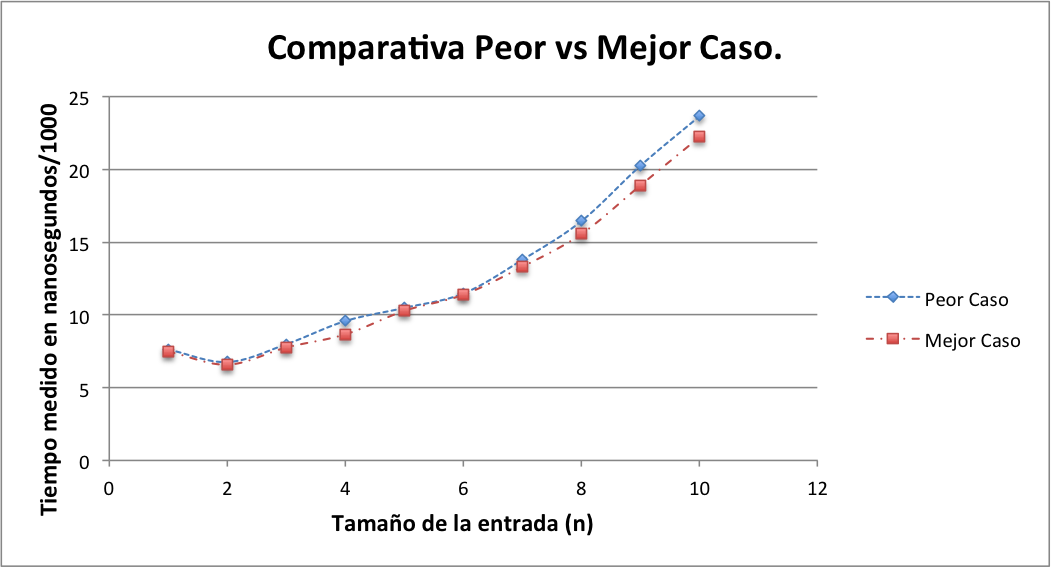
\includegraphics[width=140mm]{ejercicio3_mejorvspeor.png}
\centering
\caption{Comparativa Peor vs Mejor Caso}
\label{overflow3}
\end{figure}

\pagebreak

En el siguiente grafico pudimos realizar una acotacion de nuestro algoritmo. Por lo que pudimos acotarla por  $\bigO(e!)$ por debajo y
$\bigO(e!*(e^2))$ por arriba.

\begin{figure}[h!]
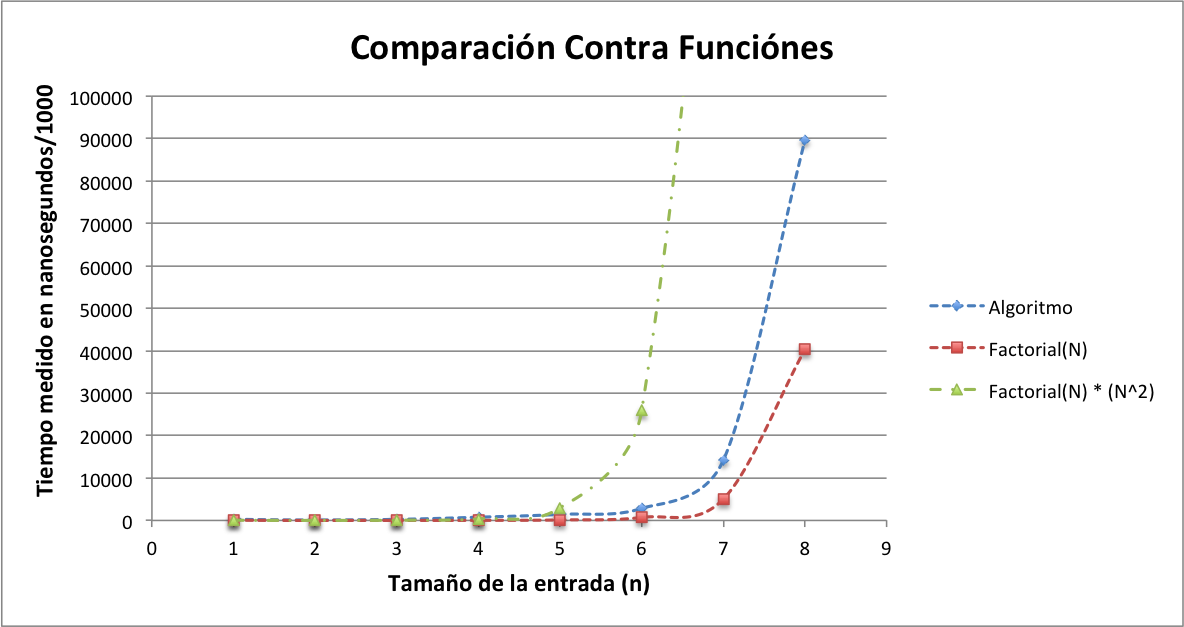
\includegraphics[width=140mm]{ejercicio3_comparacion_funciones.png}
\centering
\caption{Comparativa Contra Funcion Lineal y Cuadratica}
\label{overflow3}
\end{figure}


\pagebreak
\newpage
\section{Apendice}
\subsection{Codigo Ejercicio1}
\lstinputlisting[language=Java]{modulos/Tests_Code/ejercicio1.txt}
\subsection{Codigo Ejercicio2}
\lstinputlisting[language=Java]{modulos/Tests_Code/ejercicio2.txt}
\subsection{Codigo Ejercicio3}
\lstinputlisting[language=Java]{modulos/Tests_Code/ejercicio3.txt}
\subsection{Informe de modificaciones}
\subsubsection{Ejercicio 1}
Agregamos el enunciado del problema al principio del ejercicio.\\
Modificamos los gr\'aficos.
\subsubsection{Ejercicio 2}
Se modific\'o la secci\'on de correctitud de \'este problema.
\subsubsection{Ejercicio 3}
En el c\'odigo:

Dentro de la recursi\'on ya no chequeamos que la amiga m\'as lejana sea menor.\\
El objeto ronda calcula la amiga m\'as lejana y la suma de distancias al mismo tiempo con la funci\'on "$calcularDistancias$".\\
En el informe:

Se hicieron cambios respecto a la descripci\'on del algoritmo para explicar c\'omo funciona ahora el mismo.\\
Se modific\'o la tabla de valores en d\'onde most\'abamos la performance del mejor vs el peor caso.\\
Se agreg\'o el enunciado al principio del ejercicio.\\
Se modificaron los gr\'aficos.
\pagebreak

\end{document}
